
\subsection{Data Model}

\fmc{Modelo de Grafo - En general. Modelo PG escogido.}

\textcolor{gray}{Partes:
\begin{itemize}
    \item Justificación de por qué modelamos los datos con grafo y no de otra manera...
    \item Graph Database Model: Property graph model. Qué es un PG, por qué se elige...
    \begin{itemize}
        \item Simple/Easy to represent entities and their relationships with this data model.
        \item Good to represent dynamic data sources... relations constantly happening: modeled as edges of a graph (AMW2024 article)
        \item Good to represent evolving databases (AMW2024 article)
        \item (*) Direct way to model queries related to the search of fraud patterns: as graph patterns... query model (AMW2024 article) 
        \item Expressiveness of queries.
        \item Heuristics and indexing techniques that can be applied only if we operate in the domain of graphs: graph pattern matching and other optimizations... "translations of graphs into relations are unnatural and can not take advantage of graph-specific heuristics" (article \cite{PG-Graphs-at-a-time-GraphQL-QueryLanguage}: graph-at-a-time article).
    \end{itemize}
    \item Graph Database System: Neo4j. Otras opciones (relational database), por qué se elige...
    \item 
    \item Diferentes opciones
    \item Definir primero en general y luego definir la especificación en el caso del banco
\end{itemize}
References:
    \begin{itemize}
        \item PG: \cite{PG-angles2017foundations, PG-angles2018propertyGraphDatabaseModel, PG-Graphs-at-a-time-GraphQL-QueryLanguage, PG-exampleUsageSimeonovski}
        \item Graph Databases: \textcolor{blue}{\cite{GDB-angles2008survey, GDB-kumar2015graph}}
    \end{itemize}
}




\fmc{TODO: Describir el data model - como "Continuously evolving data graph" modelado como PG en el contexto de graph database. Poner todo como conjunto. Separación y razón de la separación del modelo en stable y volatile PGs.}
\textcolor{gray}{
Regarding the data model, the new nature of data requires a de facto new database paradigm
-continuously evolving databases- where data can be both stable and volatile. Even though
evolving databases can be implemented according to any approach, graph databases seem
especially well suited here [1, 2]. Indeed, the natural way to process evolving graphs as streams
of edges gives insights on how to proceed in order to maintain dynamic graph databases. Hence,
we consider that a suitable data model is a continuously evolving data graph, a graph having
persistent (stable) as well as non persistent (volatile) relations. Stable relations correspond
to edges occurring in standard graph databases while volatile relations are edges arriving indata streams during a set time interval. Once this time interval is over, the relations are not
longer valid so that there is no need to store them in the (stable) graph database. However,
when required -as for further legal or auditing purposes- timestamped occurrences of volatile
relations can be kept in a log file. Volatile relations induce subgraphs that exist only while the
relations are still valid. Without loss of generality, in this work we consider property graphs
(PG) [3, 4] as the basic reference data model. As an example, Figure 1a depicts part of a schema
of a PG database where stable relations correspond to the data that a bank typically gathers
on its issued cards, ATMs (Automated Teller Machines) network, etc. Volatile relations model
the interaction between cards and ATM entities}


\textcolor{blue}{In the context of our work we could see the data we are considering to be both static and streaming data, as we are considering a bank system application that contains all the information related to it on the cards, clients\dots, and that it is receiving the streaming of transactions that happens on it.
More specifically, the static data can be thinked of the classical bank database data, that is, the data a bank typically gathers on its issued cards, clients, accounts, ATMs\dots. Whereas as the streaming data we can consider the transactions the clients of the bank produce with their cards on ATMs, PoS\dots that reach the bank system.
Therefore, due to this nature of the data, we consider a \emph{continuously evolving database} paradigm, where data can be both stable and volatile. Even though 
evolving databases can be implemented according to any approach, graph databases seem especially well suited here \textcolor{blue}{\cite{angles2008survey, kumar2015graph}}. 
% TODO: PONER REFERENCIAS
% TODO: PONER + RAZONES?
}


The property graph data model consists of two sub property graphs: a stable and a volatile property graph. On the one hand, the stable is composed of the static part of the data that a bank typically gathers such as information about its clients, cards, ATMs (Automated Teller Machines). 
On the other hand, the volatile property graph models the transaction operations, which defines the most frequent and reiterative kind of interaction between entities of the data model.\\
The main difference and the main reason for this separation is the semantics with which we intentionally define each of the subgraphs: the stable will be understood like a fixed static bank database, whereas the volatile will be understood as the data model to define the transactions, as continuous interactions between the entities of the model, which will not be permanently saved, but instead, only for a certain window of time under the mission of detecting anomalous bank operations. Note that we will only model the transaction interaction in the volatile subgraph, only letting them occur here.
This separation will allow us to have a really simple and light property graph schema single-centered on the transactions with the minimal needed information (mostly identifiers of the entities a transaction links) and another, the stable, acting as a traditional bank database schema, from which to obtain the information details of the entities.

\fmc{Poner diferenciación entre Stable and Volatile PG. Por qué separamos el modelo en 2. Mostrar el PG completo conjunto.}

This property graph is a \emph{continuously evolving data graph}, which has a persistent (\emph{stable}) as well as non persistent (\emph{volatile}) relations. Stable relations correspond to edges occurring in standard graph databases while volatile relations are edges arriving in data streams during a set time interval. 

\fmc{Modelo de Grafo - Diseño de nuestro PG.}
\subsubsection*{Property Graph Data Model Design}

In what follows we describe the design of the Property Graph taken as our data model. Due to the confidential and private nature of bank data, it was impossible to find a real bank dataset nor a real bank data model. In this regard, we developed our own proposal of a bank database model taking as standard reference the \emph{Wisabi Bank Dataset}\footnote{https://www.kaggle.com/datasets/obinnaiheanachor/wisabi-bank-dataset}, which is a fictional banking dataset publicly available in the Kaggle platform. 

The proposed property graph data model is represented in Figure \ref{img:pg-complete}, consisting on both the stable and volatile property subgraphs merged. The details on both the stable and volatile property subgraphs are given next.

\begin{figure}[h]
  \centering
  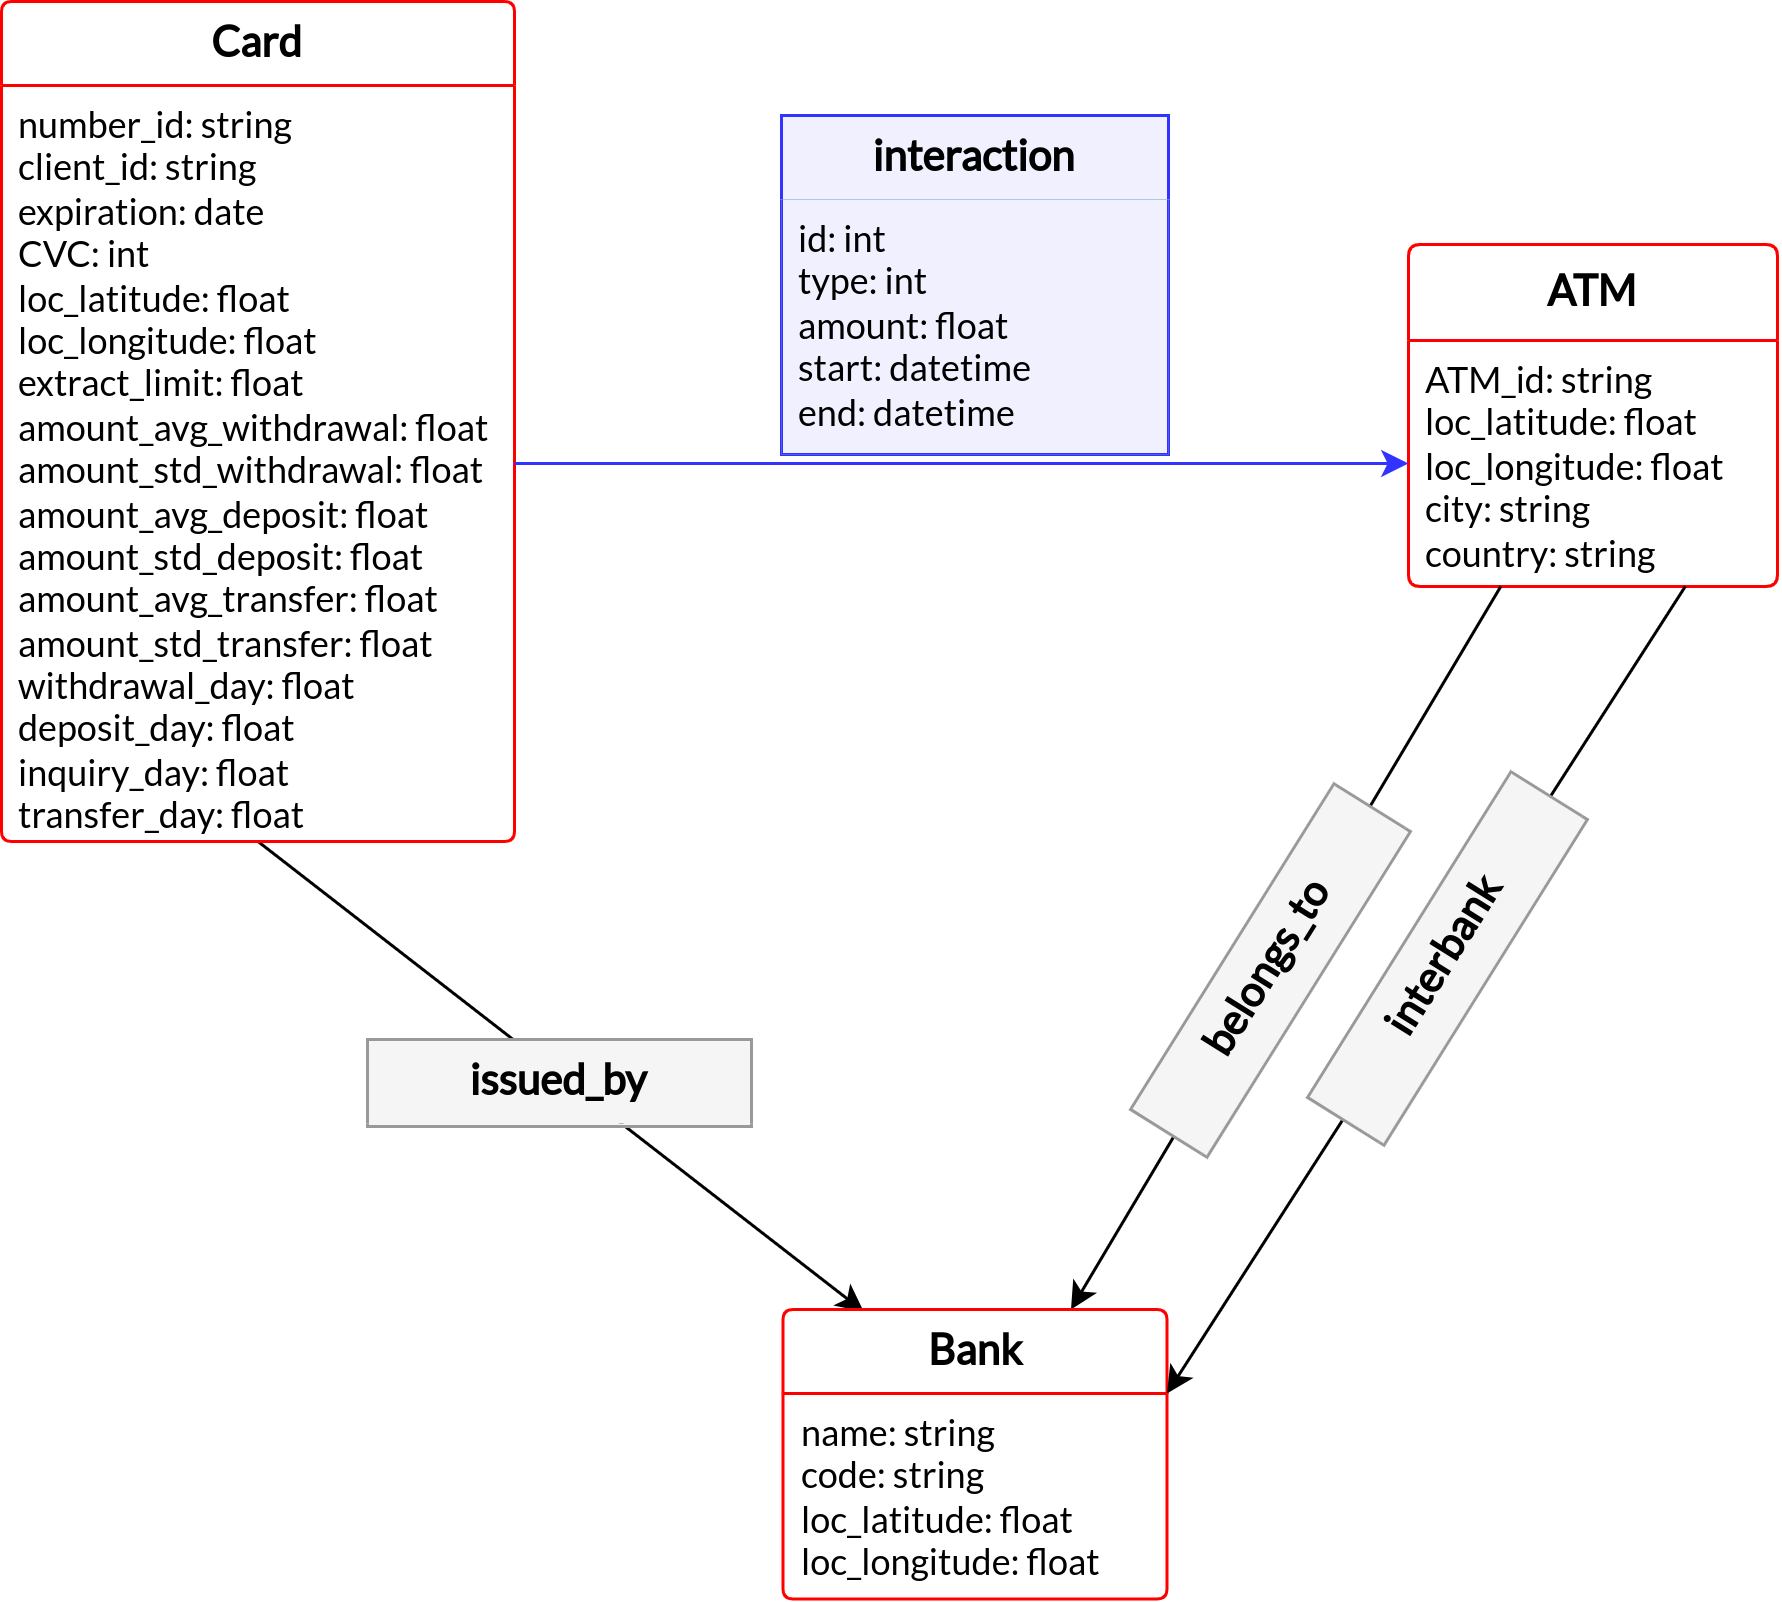
\includegraphics[scale = 0.7]{images/1-DataModel/PG-behavior-complete.png}
  \caption{Complete Property Graph Data Model}
  \label{img:pg-complete}
\end{figure}

\paragraph*{Stable Property Graph\\}\label{section:stable-pg}

Taking into account the reference dataset model, we designed a simplified version, as shown in Figure \ref{img:pg-stable-def}, with the focus on representing and modeling card-ATM interactions. On it, the defined entities, relations and properties modeling the bank database are reduced to the essential ones, which, we believe are enough to create a relevant and representative bank data model sufficient for the purposes of our work. Another option for the property graph data model representing a more common bank data model could be the one we defined in Figure \ref{img:pg-stable-big}, which intents to capture the data that a bank system database typically gathers. It consists of a more complete and possibly closer to reality data model, although unnecessarily complex for our objectives. 

\begin{figure}[h]
  \centering
  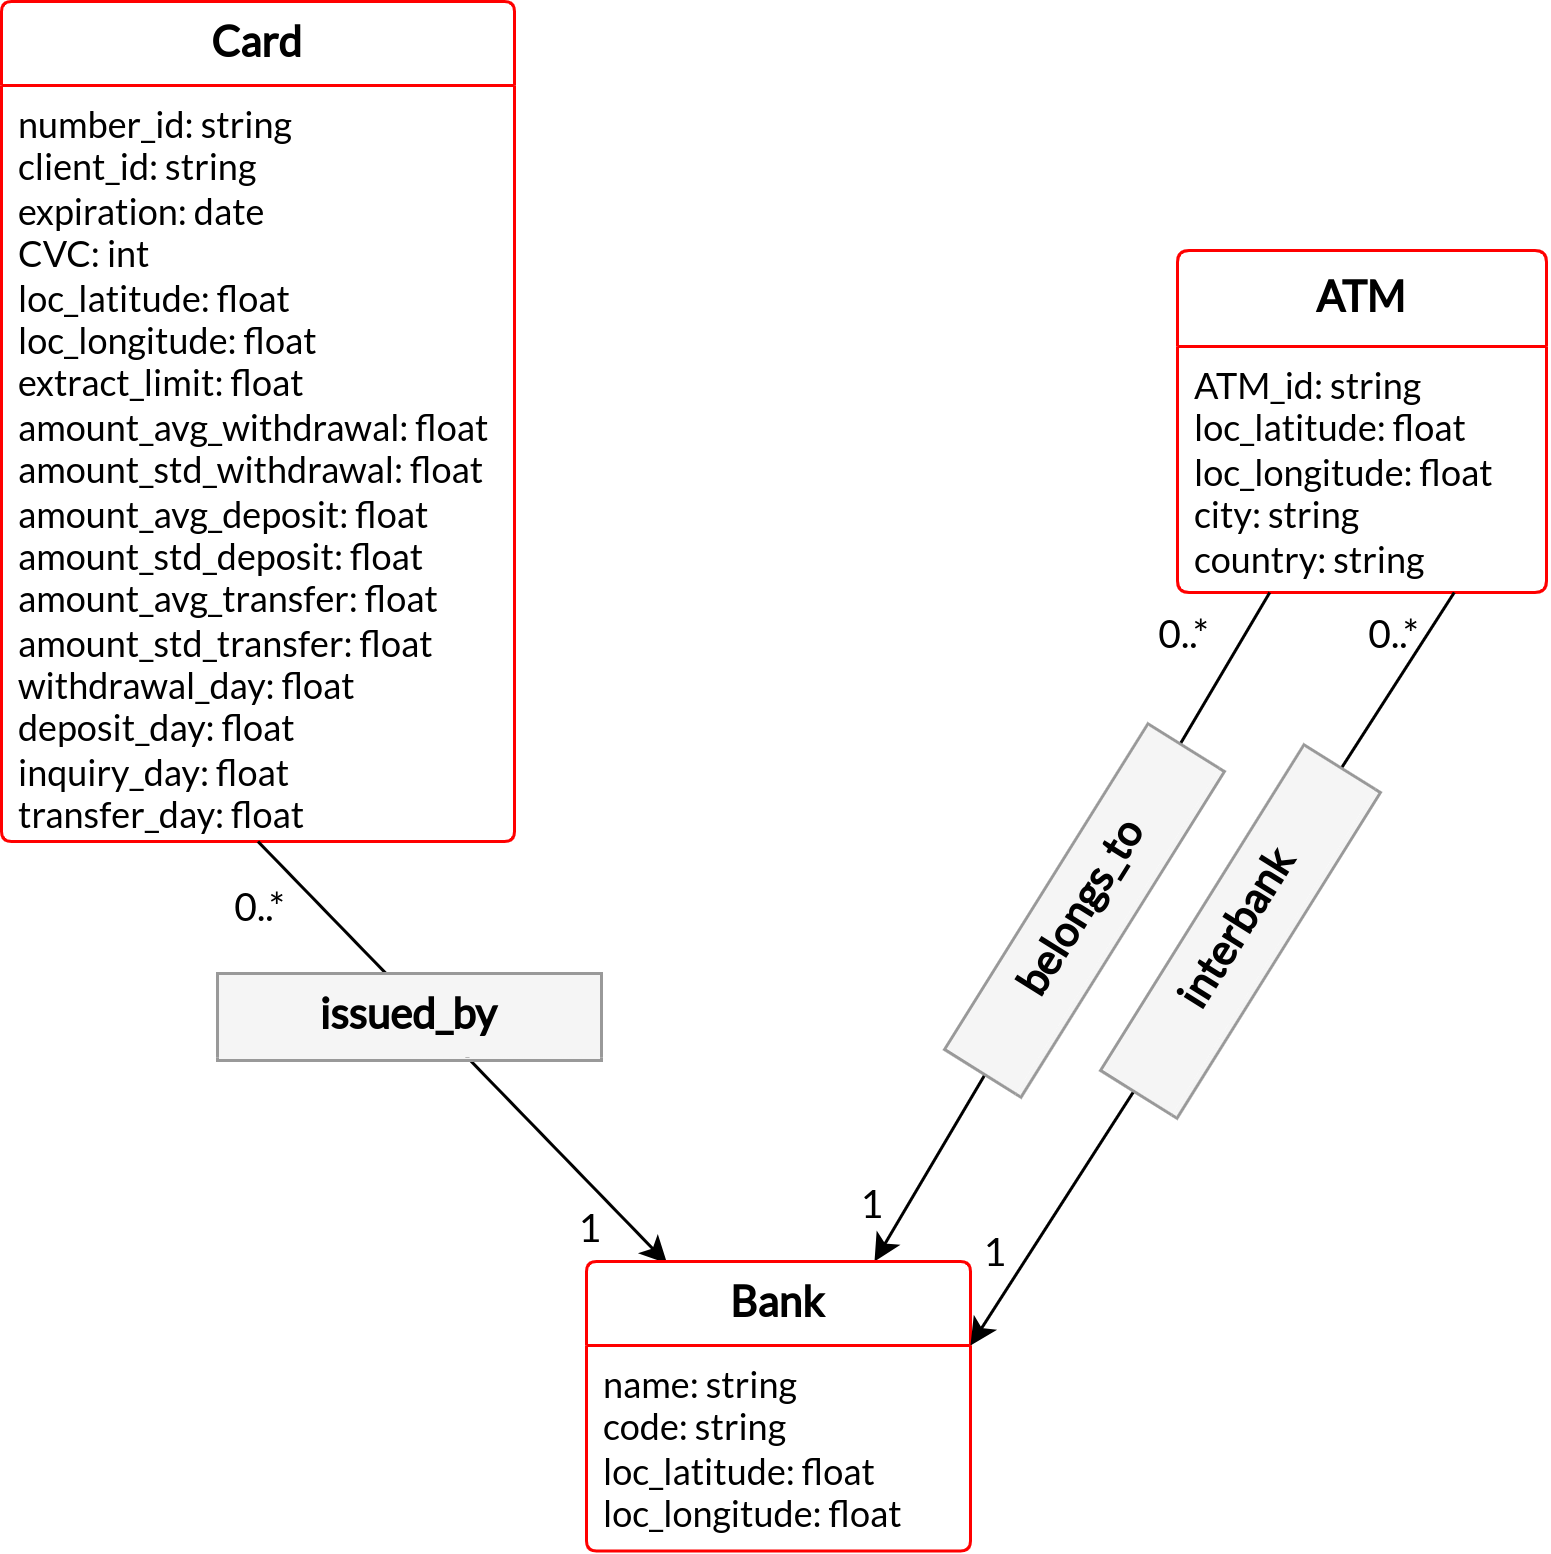
\includegraphics[scale = 0.7]{images/1-DataModel/PG-stable-behavior-cards.png}
  \caption{Stable Property Graph Data Model}
  \label{img:pg-stable-def}
\end{figure}

As a result, our definitive stable property graph model contains three node entities: Bank, Card and ATM, and three relations: \texttt{issued\_by} associating Card entities with the Bank entity, and \texttt{belongs\_to} and \texttt{interbank} associating the ATM entities with the Bank entity. 

% Bank
The Bank entity represents the bank we are considering in our system. Its properties consist
on the bank \emph{name}, its identifier \emph{code} and the location
of the bank headquarters, expressed in terms of \emph{latitude} and \emph{longitude}
coordinates, as seen in Table \ref{table:bank-node-properties}.
  
\begin{table}[H]
    \centering
      \begin{tabular}{|l|l|}
      \hline
      \textbf{Name}        & \textbf{Description and value}                                      \\ \hline
      \texttt{name}         & Bank name                                                 \\ \hline
      \texttt{code}         & Bank identifier code                                      \\ \hline
      \texttt{loc\_latitude}  & Bank headquarters GPS-location latitude                   \\ \hline
      \texttt{loc\_longitude} & Bank headquarters GPS-location longitude                  \\ \hline
      \end{tabular}
    \caption{Bank node properties}
    \label{table:bank-node-properties}
\end{table}

\fmc{Note that, from the beginning we were considering more than 1 bank entity. This lead to consider the creation of this entity, which now as only 1 bank is considered it may not be needed anymore, being able to reformulate and simplify the model. However, it is left since we considered it appropiate to be able to model the different kinds of ATMs a bank can have with different relation types instead of with different ATM types.}

The ATM entity represents the Automated Teller Machines (ATM) that either belong to the bank's network or that the bank can interact with.
% Potential possible generalization of the ATM entity to a POS entity
For the moment, this entity is understood as the classic ATM, however note that this entity could be potentially generalized to a Point Of Sale (POS) entity, allowing a more general kind of interactions apart from the current Card-ATM interaction, where also point-of-sale terminal transactions could be included apart from the ATM ones. 
\fmc{Also online / card not present (CNP) transactions?}
\fmc{El hecho de que se podría extender a la detección de otro tipo de fraude como el de PoS (Point of Sale) comentarlo también en otro apartado más visible y/o también el las conclusiones...}
We distinguish two different kinds of ATMs, depending on their relation with the bank:
\begin{itemize}
  \item Internal ATMs: ATMs owned and operated by the bank. They are fully integrated within the
  bank's network. Modeled with the \texttt{belongs\_to} relation.
  \item External ATMs: These ATMs, while not owned by the bank, are still accessible for the bank
  customers to perform transactions. Modeled with the \texttt{interbank} relation. 
\end{itemize}

Both types of ATMs are considered to be of the same type of ATM node. Their difference
is modeled as their relation with the bank instance: \texttt{belongs\_to} for the internal ATMs and \texttt{interbank} for the external ATMs.

\begin{table}[H]
    \centering
    \begin{tabular}{|l|l|}
    \hline
    \textbf{Property}        & \textbf{Description}                                      \\ \hline
    \texttt{ATM\_id}      & ATM unique identifier                             \\ \hline
    \texttt{loc\_latitude}  & ATM GPS-location latitude           \\ \hline
    \texttt{loc\_longitude} & ATM GPS-location longitude          \\ \hline
    \texttt{city}         & ATM city location                         \\ \hline
    \texttt{country}      & ATM country location                       \\ \hline
    \end{tabular}
    \caption{ATM node properties}
    \label{table:atm-node-properties}
\end{table}

The ATM node type properties consist on the ATM unique identifier \emph{ATM\_id}, its location, expressed in terms of \emph{latitude} and \emph{longitude} coordinates, and the \emph{city} and 
\emph{country} in which it is located, as seen in Table \ref{table:atm-node-properties}.
Note that the last two properties are somehow redundant, considering that location coordinates
are already included. In any case both properties are maintained since their inclusion provides a more explicit and direct description of the location of the ATMs, which will be of special interest for some of the card anomalous patterns that will be considered.\\

Finally, the Card node type represents the cards of the clients in the bank system. The Card node type properties, as depicted in Table
\ref{table:card-node-properties}, consist on the card unique 
identifier \emph{number\_id}, the associated client unique identifier \emph{client\_id}, the card validity expiration date \emph{expiration}, the Card Verification Code, \emph{CVC}, the coordinates of the associated client habitual residence address \emph{loc\_latitude} and 
\emph{loc\_longitude} and the \emph{extract\_limit} property, which represents the limit on the amount of money it can be extracted with the card on a single withdrawal, related with the the amount of money a person owns. These last two properties are of special interest for some future card fraud patterns to be considered. In the first case related with interactions far from the client's habitual residence address and in the second with unusually frequent or very high expenses interactions.

Finally it contains the properties related with the \emph{behavior} of the client, representing the usual comportment of a client in regard with its ATM usage: \emph{amount\_avg\_withdrawal}, \emph{amount\_std\_withdrawal}, \emph{amount\_avg\_deposit}, 
\emph{amount\_std\_deposit}, \emph{amount\_avg\_transfer},  \emph{amount\_std\_transfer}, \emph{withdrawal\_day}, \emph{deposit\_day}, \emph{transfer\_day} and \emph{inquiry\_day}.
They are metrics representing the behavior of the owner of the Card, and they are included as properties as we think they could be of interest to allow the detection of some kinds of anomalies related with anomalous client's behavior in the future.

\begin{table}[H]
    \centering
    \begin{tabular}{|l|l|}
    \hline
    \textbf{Name}        & \textbf{Description and value}                                          \\ \hline
    \texttt{number\_id}   & Card unique identifier                               \\ \hline
    \texttt{client\_id}   & Client unique identifier                               \\ \hline
    \texttt{expiration}   & Card validity expiration date                      \\ \hline
    \texttt{CVC}          & Card Verification Code                                      \\ \hline
    \texttt{extract\_limit} & Card money amount extraction limit    \\ \hline
    \texttt{loc\_latitude}  & Client's habitual address GPS-location latitude                         \\ \hline
    \texttt{loc\_longitude} & Client's habitual address GPS-location longitude                        \\ \hline
    \end{tabular}
    \caption{Card node properties}
    \label{table:card-node-properties}
\end{table}

The client is completely anonymized in the system (no name, surname, age, or any other confidential details) by using only a \emph{client\_id}. Currently, \emph{client\_id} is included in the Card node type for completeness. However, it could be omitted for simplicity, as we assume a one-to-one relationship between card and client for the purposes of our work -- each card is uniquely associated with a single client, and each client holds only one card. Thus, the \emph{client\_id} is not essential at this stage but is retained in case the database model is expanded to support clients with multiple cards or cards shared among different clients.

\begin{figure}[h]
  \centering
  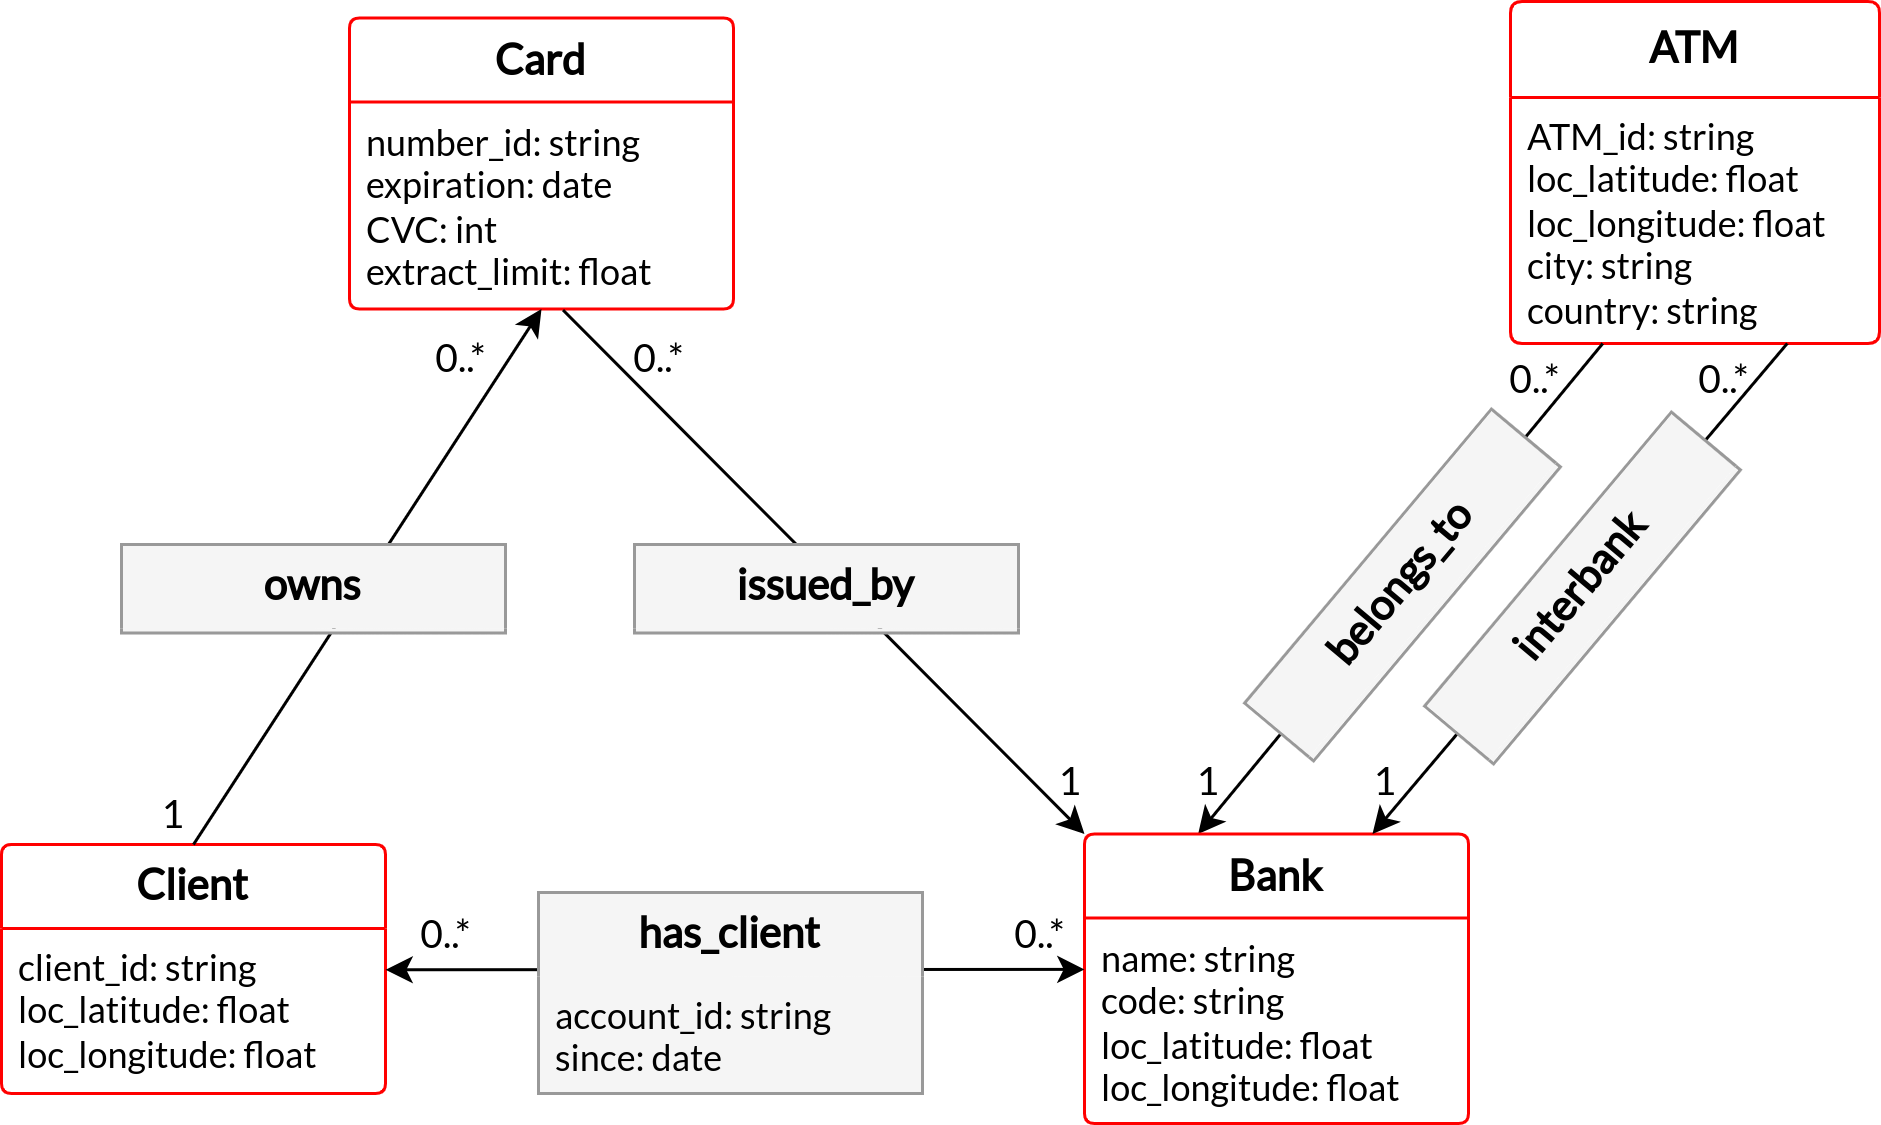
\includegraphics[scale = 0.7]{images/1-DataModel/PG-stable-edit-cardinal.png}
  \caption{Alternative - Complex Stable Property Graph Data Model}
  \label{img:pg-stable-big}
\end{figure}

\fmc{Describir el modelo más complejo? / el inicial?}

The more complex alternative model, shown in Figure \ref{img:pg-stable-big}, contains four entities: Bank, ATM, Client and Card with their respective properties, and the corresponding relationships between them. The relations are: a directed relationship from Client to Card \texttt{owns} representing that a client can own multiple credit cards and that a card is owned by a unique client, then a bidirectional relation \texttt{has\_client} between Client and Bank; representing bank accounts of the clients in the bank. The relation between Card and Bank to represent that a card is \texttt{issued\_by} the bank, and that the bank can have multiple cards issued. Finally, the relations \texttt{belongs\_to} and \texttt{interbank} between the ATM and Bank entities, representing the two different kinds of ATMs depending on their relation with the bank; those ATMs owned and operated by the bank and those that, while not owned by the bank, are still accessible for the bank customers to perform transactions.

This model allows a more elaborated representation of what a bank system database is. As it can be seen it represents clients as an independent entity from the Card entity, and it also allows to represent bank accounts through the relation between the Client and Bank entities. 

\fmc{Quitar esto ya?}
\ad{Sí, todo lo que no te sirva quítalo o comentalo ya, guarda el texto por si te puede llegar a hacer falta pero ya ve avanzando en la versión más definitiva del documento.}
\textcolor{gray}{
On the final version of the model, we decided to remove the Client entity and to merge it inside the Card entity. For this, all the Client properties were included in the Card entity. In the complete data model schema (Figure \ref{img:pg-stable-big}) the Client entity was defined with three properties: the identifier of the client and the GPS coordinates representing the usual residence of the client. This change is done while preserving the restriction of a Card belonging to a unique client the same way it was previously done with the relation between Card and Client \texttt{owns} in the complete schema, which now is therefore removed.} \\
% Account relation removed
\textcolor{gray}{
Another derived consequence of this simplification is the removal of the other relation that the Client entity had with other entities: the \texttt{has\_client} relation between Client and Bank, which was made with the intention of representing the bank accounts between clients and banks. Maintaining a bank account would imply having to consistently update the bank account state after each transaction of a client, complicating the model. Nevertheless, we eliminate the bank account relation, since its removal is considered negligible and at the same time helpful for the simplification of the model needed for the purposes of our work. % Properties included with the purpose of detecting frauds 
However, for the sake of completeness the property \textit{extract\_limit} is introduced in the Card entity, representing a money amount limit a person can extract, which will be related with the amount of money a person owns. This will allow the detection of anomalies related with frequent or very high expenses. Other properties that are included with the purpose of allowing the detection of some other kinds of anomalies are the GPS coordinates and the client's \emph{behavior} properties. The GPS coordinates are added in the ATM and Card entities, in the first case referring to the geolocation of each specific ATM and in the last case referring to each specific client address geolocation. The client's \emph{behavior} properties are added in the Card entity. They are metrics representing the behavior of the owner of the Card, and they are included as properties as we think they could be of interest to allow the detection of some kinds of anomalies in the future.}


\paragraph*{Volatile Property Graph\\}\label{section:volatile-pg}

The volatile property graph consists on an abstraction of the property graph model to describe the interactions between the cards and the ATMs in the bank system (see it on Figure \ref{img:pg-volatile}). These interactions are going to be continuously occurring and arriving to our system as data stream.

This property graph is a subgraph of the original bank property graph model. It contains the Card and ATM entities with the minimal information needed to identify them -- \emph{number\_id} and \emph{ATM\_id}, Card and ATM identifiers, respectively -- between which the interaction occurs, along with additional details related to the interaction. Those identifiers are enough to be able to recover, if needed, the whole information about the specific Card or ATM entity in the stable property graph.

\begin{figure}[h]
    \centering
    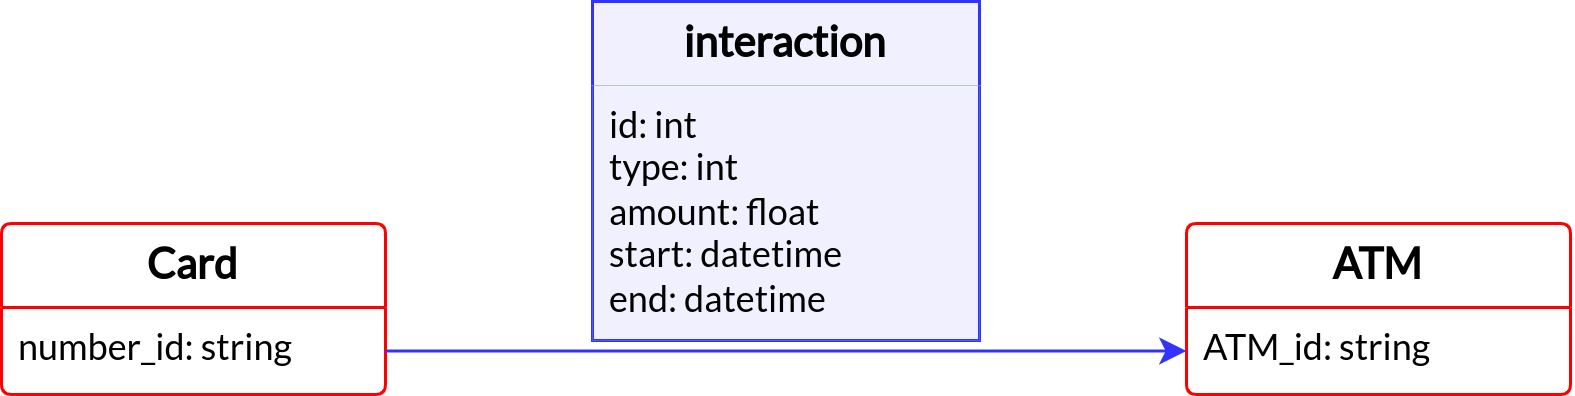
\includegraphics[scale = 0.8]{images/1-DataModel/schema-volatile.png}
    \caption{Volatile Property Graph Data Model}
    \label{img:pg-volatile}
\end{figure}

Finally, it contains the \emph{interaction} relationship between the Card and the ATM nodes. The \emph{interaction} relation contains as properties: \emph{id} as the interaction unique identifier, \emph{type} which describes the type of the interaction (withdrawal, deposit, balance inquiry or transfer), \emph{amount} describing the amount of money involved in the interaction in the local currency considered, and finally, \emph{start} and \emph{end} which define the interaction \emph{datetime} start and end moments, respectively. 

\fmc{TODO: Poner tabla de propiedades de la relacion interaction como con las propiedades de las entities: Bank, Card y ATM}

\fmc{TODO: Poner aqui lo de interaction start y end, la diferenciación y el por qué. En lugar de hacerlo en el apartado de la generación de transacciones}

\begin{comment}
\begin{itemize}
  \item[-] transaction\_id: Unique identifier for each transaction in the database.
  \item[-] transaction\_start: Datetime when the transaction started. Format: DD/MM/YYYY HH:MM (ex. 1/1/2022 4:50).
  \item[-] transaction\_end: Datetime when the transaction was completed. Format: DD/MM/YYYY HH:MM (ex. 1/1/2022 4:54).
  \item[-] transaction\_amount: Amount of money involved in the transaction.
\end{itemize}

\begin{figure}[H]
    \centering
    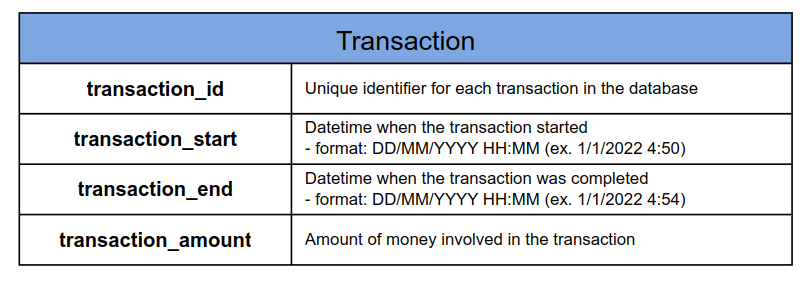
\includegraphics[scale = 0.40]{images/transaction.png}
    \caption{Transaction relation attributes}
    \label{img:pg-stable}
\end{figure}

\end{comment}

\iffalse


\fi
